%-------------------------------------------------------------------------
% Design Project Input/Output Module Description
%-------------------------------------------------------------------------

\clearpage
\section{Printer Output Module}
\label{sec-output-printer}

This printer output module enables your IoT device to print a paper copy
of collected/processed data for the end-user. The printer is a thermal
receipt printer, similar to what is used in most retail stores. A
thermal printer works by selectively heating special thermochromic
paper. Heated sections of paper turn black, creating the desired text or
image, e.g., a barcode.

We'll be using the Arduino to control the printer. However, because the
printer's thermal print head needs to be hot to work, it requires its
own power supply. The printer comes with its own wall-wart power supply,
which you should plug into the barrel connector to screw-down terminal
converter. Ensure that positive (red) is connected to the \texttt{+} and
negative (black) is connected to the \texttt{-}. The printer has small
plugs on the bottom: a 2-pin (power) and a 3-pin (data). Connect the
power cable to the 2-pin plug (red/black) and hook that up to the barrel
connector converter. The data cable connects to the Arduino for control.
Green to digital pin 5, yellow to digital pin 6, and black to ground.

%\begin{center}
%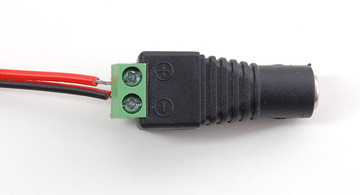
\includegraphics[width=2in]{components_poweradapt.jpg}
%\end{center}

\begin{center}
  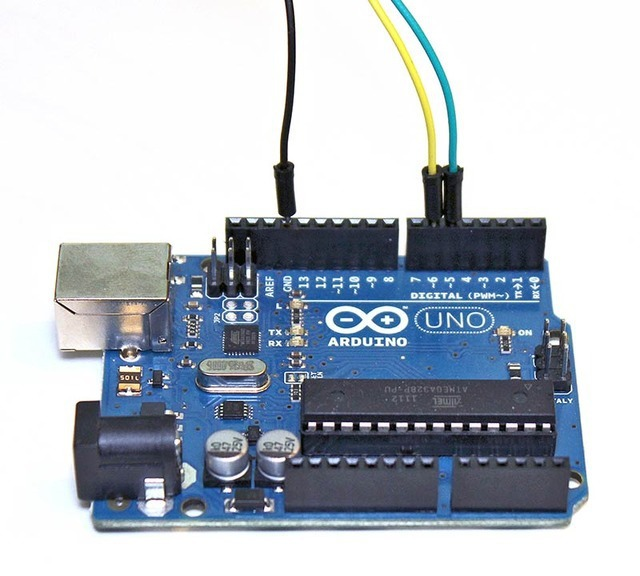
\includegraphics[width=0.4\tw]{components_printer-wiring.jpg}
\end{center}

\begin{minipage}[t]{0.49\tw}
  \vspace{0.0in}
  \begin{Verbatim}[gobble=3,fontsize=\small]
      #include "SoftwareSerial.h"
      #include "Adafruit_Thermal.h"
      #include <avr/pgmspace.h>

      int printer_RX_Pin = 5;
      int printer_TX_Pin = 6;

      Adafruit_Thermal
        printer(printer_RX_Pin, printer_TX_Pin);
  \end{Verbatim}
\end{minipage}
\hfill
\begin{minipage}[t]{0.49\tw}
  \vspace{0.15in}
  \begin{Verbatim}[gobble=3,fontsize=\small]
      void setup() {
        Serial.begin(9600);
        pinMode(7, OUTPUT);
        digitalWrite(7, LOW);
        printer.begin();
      }

      void loop() {
        print.println("Hello World!")

        // Set text justification (left, center, right)
        // Accepts 'L', 'C', 'R'
        printer.justify('C');
        printer.println("This Text Center Justified");

        // Set type size, accepts 'S', 'M', 'L'
        printer.setSize('M');
        printer.println("Medium Text");

        printer.feed(1);
      }
  \end{Verbatim}
\end{minipage}


